\begin{frame}
	\frametitle{\ejerciciocmd}
	\framesubtitle{Enunciado}
	\textbf{
		Dadas las siguientes reacciones:
\begin{itemize}
    \item \ce{I2(g) + H2(g) -> 2 HI(g)}~~~$\Delta H_1 = \SI{-0,8}{\kilo\calorie}$
    \item \ce{I2(s) + H2(g) -> 2 HI(g)}~~~$\Delta H_2 = \SI{12}{\kilo\calorie}$
    \item \ce{I2(g) + H2(g) -> 2 HI(ac)}~~~$\Delta H_3 = \SI{-26,8}{\kilo\calorie}$
\end{itemize}
Calcular los parámetros que se indican a continuación:
\begin{description}%[label={\alph*)},font={\color{red!50!black}\bfseries}]
    \item[\texttt{a)}] Calor molar latente de sublimación del yodo.
    \item[\texttt{b)}] Calor molar de disolución del ácido yodhídrico.
    \item[\texttt{c)}] Número de calorías que hay que aportar para disociar en sus componentes el yoduro de hidrógeno gas contenido en un matraz de \SI{750}{\cubic\centi\meter} a \SI{25}{\celsius} y \SI{800}{\torr} de presión.
\end{description}
\resultadocmd{\SI{12,8}{\kilo\calorie}; \SI{-13,0}{\kilo\calorie}; \SI{12,9}{\calorie}}

		}

\end{frame}

\begin{frame}
	\frametitle{\ejerciciocmd}
	\framesubtitle{Resolución (\rom{1}): Obtención de la $\Delta H$ de reacción}
	\begin{overprint}
		\onslide<1>
			Para poder utilizar la ecuación de Van't Hoff, que nos relaciona el valor de la constante de equilibrio a dos temperaturas diferentes primeramente necesitamos $\Delta H$ de reacción. Si observamos la expresión:
			$$
				\ln K = -\frac{\Delta H}{R\vdot T} + \frac{\Delta S^0}{R}
			$$
			Nos damos cuenta de que podemos usar los datos de la tabla para representar $\ln K$ frente a $T^{-1}$. En la siguiente tabla realizamos las operaciones necesarias para la representación:
			\begin{center}
				\begin{tabular}{SSSS}
					\toprule
						{$T~(\si{\kelvin})$} & {$T^{-1}~(\si{\per\kelvin})$} & {K} & {$\ln K$} \\
					\midrule
						 800 & 12.50e-4 & 9.1e2  &  6.81 \\
						 850 & 11.80e-4 & 1.7e2  &  5.14 \\
						 900 & 11.10e-4 & 4.2e1  &  3.74 \\
						 950 & 10.50e-4 & 1.0e1  &  2.30 \\
						1000 & 10.00e-4 & 3.2e0  &  1.16 \\
						1050 &  9.52e-4 & 1.0e0  &  0.00 \\
						1100 &  9.09e-4 & 3.9e-1 & -0.94 \\
						1170 &  8.50e-4 & 1.2e-1 & -2.12 \\
					\bottomrule
				\end{tabular}
			\end{center}
		\onslide<2>
			% GNUPLOT: LaTeX picture with Postscript
\begingroup
  \makeatletter
  \providecommand\color[2][]{%
    \GenericError{(gnuplot) \space\space\space\@spaces}{%
      Package color not loaded in conjunction with
      terminal option `colourtext'%
    }{See the gnuplot documentation for explanation.%
    }{Either use 'blacktext' in gnuplot or load the package
      color.sty in LaTeX.}%
    \renewcommand\color[2][]{}%
  }%
  \providecommand\includegraphics[2][]{%
    \GenericError{(gnuplot) \space\space\space\@spaces}{%
      Package graphicx or graphics not loaded%
    }{See the gnuplot documentation for explanation.%
    }{The gnuplot epslatex terminal needs graphicx.sty or graphics.sty.}%
    \renewcommand\includegraphics[2][]{}%
  }%
  \providecommand\rotatebox[2]{#2}%
  \@ifundefined{ifGPcolor}{%
    \newif\ifGPcolor
    \GPcolortrue
  }{}%
  \@ifundefined{ifGPblacktext}{%
    \newif\ifGPblacktext
    \GPblacktexttrue
  }{}%
  % define a \g@addto@macro without @ in the name:
  \let\gplgaddtomacro\g@addto@macro
  % define empty templates for all commands taking text:
  \gdef\gplbacktext{}%
  \gdef\gplfronttext{}%
  \makeatother
  \ifGPblacktext
    % no textcolor at all
    \def\colorrgb#1{}%
    \def\colorgray#1{}%
  \else
    % gray or color?
    \ifGPcolor
      \def\colorrgb#1{\color[rgb]{#1}}%
      \def\colorgray#1{\color[gray]{#1}}%
      \expandafter\def\csname LTw\endcsname{\color{white}}%
      \expandafter\def\csname LTb\endcsname{\color{black}}%
      \expandafter\def\csname LTa\endcsname{\color{black}}%
      \expandafter\def\csname LT0\endcsname{\color[rgb]{1,0,0}}%
      \expandafter\def\csname LT1\endcsname{\color[rgb]{0,1,0}}%
      \expandafter\def\csname LT2\endcsname{\color[rgb]{0,0,1}}%
      \expandafter\def\csname LT3\endcsname{\color[rgb]{1,0,1}}%
      \expandafter\def\csname LT4\endcsname{\color[rgb]{0,1,1}}%
      \expandafter\def\csname LT5\endcsname{\color[rgb]{1,1,0}}%
      \expandafter\def\csname LT6\endcsname{\color[rgb]{0,0,0}}%
      \expandafter\def\csname LT7\endcsname{\color[rgb]{1,0.3,0}}%
      \expandafter\def\csname LT8\endcsname{\color[rgb]{0.5,0.5,0.5}}%
    \else
      % gray
      \def\colorrgb#1{\color{black}}%
      \def\colorgray#1{\color[gray]{#1}}%
      \expandafter\def\csname LTw\endcsname{\color{white}}%
      \expandafter\def\csname LTb\endcsname{\color{black}}%
      \expandafter\def\csname LTa\endcsname{\color{black}}%
      \expandafter\def\csname LT0\endcsname{\color{black}}%
      \expandafter\def\csname LT1\endcsname{\color{black}}%
      \expandafter\def\csname LT2\endcsname{\color{black}}%
      \expandafter\def\csname LT3\endcsname{\color{black}}%
      \expandafter\def\csname LT4\endcsname{\color{black}}%
      \expandafter\def\csname LT5\endcsname{\color{black}}%
      \expandafter\def\csname LT6\endcsname{\color{black}}%
      \expandafter\def\csname LT7\endcsname{\color{black}}%
      \expandafter\def\csname LT8\endcsname{\color{black}}%
    \fi
  \fi
    \setlength{\unitlength}{0.0500bp}%
    \ifx\gptboxheight\undefined%
      \newlength{\gptboxheight}%
      \newlength{\gptboxwidth}%
      \newsavebox{\gptboxtext}%
    \fi%
    \setlength{\fboxrule}{0.5pt}%
    \setlength{\fboxsep}{1pt}%
\begin{picture}(6220.00,3960.00)%
    \gplgaddtomacro\gplbacktext{%
      \csname LTb\endcsname%%
      \put(820,652){\makebox(0,0)[r]{\strut{}$-3.0$}}%
      \csname LTb\endcsname%%
      \put(820,960){\makebox(0,0)[r]{\strut{}$-2.0$}}%
      \csname LTb\endcsname%%
      \put(820,1269){\makebox(0,0)[r]{\strut{}$-1.0$}}%
      \csname LTb\endcsname%%
      \put(820,1577){\makebox(0,0)[r]{\strut{}$0.0$}}%
      \csname LTb\endcsname%%
      \put(820,1885){\makebox(0,0)[r]{\strut{}$1.0$}}%
      \csname LTb\endcsname%%
      \put(820,2194){\makebox(0,0)[r]{\strut{}$2.0$}}%
      \csname LTb\endcsname%%
      \put(820,2502){\makebox(0,0)[r]{\strut{}$3.0$}}%
      \csname LTb\endcsname%%
      \put(820,2810){\makebox(0,0)[r]{\strut{}$4.0$}}%
      \csname LTb\endcsname%%
      \put(820,3118){\makebox(0,0)[r]{\strut{}$5.0$}}%
      \csname LTb\endcsname%%
      \put(820,3427){\makebox(0,0)[r]{\strut{}$6.0$}}%
      \csname LTb\endcsname%%
      \put(820,3735){\makebox(0,0)[r]{\strut{}$7.0$}}%
      \csname LTb\endcsname%%
      \put(932,448){\makebox(0,0){\strut{}$8.5$}}%
      \csname LTb\endcsname%%
      \put(1548,448){\makebox(0,0){\strut{}$9$}}%
      \csname LTb\endcsname%%
      \put(2165,448){\makebox(0,0){\strut{}$9.5$}}%
      \csname LTb\endcsname%%
      \put(2781,448){\makebox(0,0){\strut{}$10$}}%
      \csname LTb\endcsname%%
      \put(3398,448){\makebox(0,0){\strut{}$10.5$}}%
      \csname LTb\endcsname%%
      \put(4014,448){\makebox(0,0){\strut{}$11$}}%
      \csname LTb\endcsname%%
      \put(4630,448){\makebox(0,0){\strut{}$11.5$}}%
      \csname LTb\endcsname%%
      \put(5247,448){\makebox(0,0){\strut{}$12$}}%
      \csname LTb\endcsname%%
      \put(5863,448){\makebox(0,0){\strut{}$12.5$}}%
    }%
    \gplgaddtomacro\gplfronttext{%
      \csname LTb\endcsname%%
      \put(186,2193){\rotatebox{-270}{\makebox(0,0){\strut{}$\ln K$\quad}}}%
      \csname LTb\endcsname%%
      \put(3397,142){\makebox(0,0){\strut{}$T^{-1}~(\si{\per\kelvin})\times\num{1e4}$}}%
      \csname LTb\endcsname%%
      \put(4998,3552){\makebox(0,0)[r]{\strut{}\small$\ln K$ = -21,3267 + 2,2492$\times T^{-1}$ ($r^2$ = 0.9995)}}%
    }%
    \gplbacktext
    \put(0,0){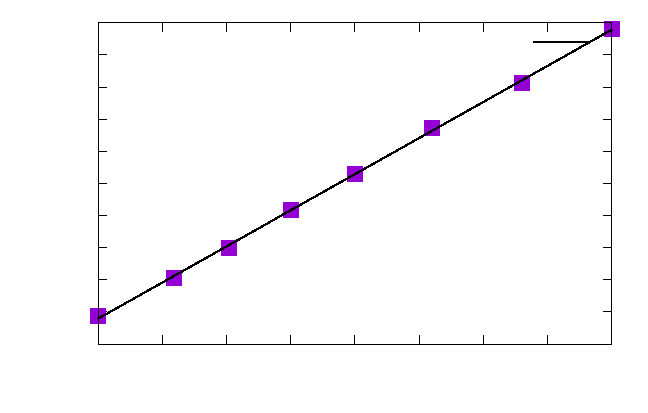
\includegraphics[width={311.00bp},height={198.00bp}]{/home/nicux/Documentos/docencia/repositorio/ejercicios/quimica_general/equilibrio/vant_hoff/figs/vant_hoff}}%
    \gplfronttext
  \end{picture}%
\endgroup

			\structure{Pendiente:} $\num{2,2492} = -\rfrac{\Delta H}{R}\times\num{1e-4}$ (recordad que la inversa de $T$ está multiplicada por \num{10000}).
			\structure{Variación de entalpía estándar de esta reacción:}
			$$
				\Delta H = -\SI{8,3145}{\joule\per\mol\per\kelvin}\times\num{2,2492}\times\num{1e4} = \SI{-1,870e5}{\joule\per\mol} = \SI{-187,0}{\kilo\joule\per\mol}
			$$ 
	\end{overprint}
\end{frame}

\begin{frame}
	\frametitle{\ejerciciocmd}
	\framesubtitle{Resolución (\rom{2}): temperatura a la que la constante de equilibrio vale \num{1e6}}
	\structure{Ecuación de Van't Hoff:}
	$$
		\ln(\frac{K_2}{K_1}) = \frac{\Delta H}{R}\vdot\left(\frac{T_2 - T_1}{T_2\vdot T_1}\right)
	$$
	Para el estado \num{1} podemos emplear cualquier valor de la tabla (p.ej. $T_1 = \SI{800}{\kelvin}$ y $K_1 = \num{910}$). Para el estado \num{2} $K_2 = \num{1e6}$.\\[.2cm]
	\structure{Despejando $T_2$:}
	$$
		T_2 = \frac{\Delta H}{\frac{\Delta H}{T_1} + R\vdot\ln(\frac{K_1}{K_2})}
	$$
	\structure{Sustituyendo:}
	$$
		T_2 = \frac{\SI{-1,870e5}{\cancel\joule\per\cancel\mol}}{\frac{\SI{-1,870e5}{\cancel\joule\per\cancel\mol}}{\SI{800}{\kelvin}} + \SI{8,3145}{\cancel\joule\per\cancel\mol\per\kelvin}\vdot\ln(\frac{\num{9,1e2}}{\num{1e6}})}
	$$
	$$
		\tcbhighmath[boxrule=0.4pt,arc=4pt,colframe=red,drop fuzzy shadow=orange]{T_2 = \SI{637}{\kelvin}}
	$$
\end{frame}
